\chapter{Event reconstruction in CMS}

While traversing the different detector layers, the particles produced in the physics collisions deposit energy in the detectors that is amplified and recorded. Most sub-detectors are capable of measuring the particle position as well as the deposited energy. Each collision event results in a series of position measurements in the different layers of the tracking detectors plus energy clusters in the calorimeter. The reconstruction algorithms takes care of ``connecting the dots'' and provide the most complete and accurate description of the event as it originated from the collision. In this task the algorithm execution time plays an important role, as the algorithms used by the reconstruction cannot be excessively resource demanding. In this chapter we will briefly describe the techniques used to reconstruct the events recorded by the CMS detector starting from the most basic objects and then moving towards the most complex ones. Finally, we describe the \emph{Particle Flow} algorithm that gives a global description of the event. At the end of the chapter we will describe in detail the hadronic tau reconstruction, which plays a fundamental role in this work, and the techniques used to measure its efficiency.

\section{Track reconstruction}

The signals recorded by the innermost sub-detector, the inner tracker ( see section \ref{sec:inner_tracker}), are used to reconstruct the trajectory and momenta of the charged particles originating from the proton collisions as well as the location (vertex) where these interactions occurred. An accurate and detailed description of the tracking algorithms can be found in Ref. \cite{cms_trk_11_01}.

The innermost part of the tracker, made of silicon pixel detectors, records the hit position together with the charge deposited in the detector. Due to the Lorentz drift the charge deposited by a ionizing particle is shared between neighboring pixels, improving the position resolution of the detector. The outer part of the tracker, made of silicon strip detectors, generally records only the $\phi$\ coordinate of the hit except for few layers where an additional strip module rotated by a 100 mrad stereo angle allows for a bi--dimensional measurement of the hit positions.

Due to huge number of hits recorded in each event, reconstructing the tracks corresponding to the hits is not trivial. The strategy adopted by the CMS collaboration employs a \emph{combinatoric track finding} (CTF) approach with very stringent requirements on the tracks, thus finding the easiest ones to reconstruct first. These requirements are progressively loosened in several iterations. After each iteration the hits used to build the tracks are removed from the pool of available hits. This procedure, called \emph{iterative tracking}, allows to achieve a very high tracking efficiency with low fake rate and acceptable resource usage. 

At the beginning of each iteration the tracks are seeded from triplets or doublets of hits in the tracker. In case of doublets an additional constraint on the beam-spot is used to reduce the fake rate. Only 2D hits are used at this stage to build track seeds. A first evaluations of the main track parameters (\pT and 3D impact parameter) is also performed at the seeding step. Track seeds not satisfying the minimal requirements for that iteration are discarded.

Track seeds are then propagated ``inwards'' (in the direction of the nominal interaction point) and ``outwards'' (in the direction of the calorimeter) the seeding layers in order to search for compatible hits that can be assigned to the track. The analytical propagator used at this stage assumes uniform magnetic field in between the two detector layers and neglects multiple scattering effects. New candidate hits are added to the track candidate and its parameters are updated by a \emph{Kalman Filter} \cite{Fruhwirth:1987fm}. Only the track candidates satisfying a certain fit quality (evaluated with the $\chi^2$) are retained. This process, known as \emph{track finding}, is repeated until the innermost and outermost layers of the tracker are reached by the track propagation. During this process the Kalman Filter retains only the latest and most accurate evaluation of the track parameters and the addition of a new hit does not require re-evaluating the full trajectory, saving a large amount of computing time. Track candidates emerging from this process are cleaned, merging those candidates sharing the majority of the hits. Mutually-exclusive hits (hits belonging to the same detector layer) are arbitrated according to the $\chi^2$\ goodness of the track fit.

Track candidates found during the track finding step are then fitted by the means of Kalman filter and smoother. This choice is as accurate as a standard fit, but more effective from the computational point of view. Trajectory parameters are evaluated both starting from the innermost hit in the tracker and from the outermost one and then averaged, avoiding any bias due to the recursive nature of the Kalman Filters. During this process the more refined Runge-Kutta propagator is used to take into account un--homogeneities of the magnetic field and the effect of materials. Track candidates are finally selected according to the quality of the fit. Hits belonging to the tracks produced by this last step are removed from the collection of available hits and a new iteration with different seeding conditions and track requirements begins. 

A total of six iterations is performed on each event, the first ones are aimed at reconstructing most of the tracks originating from the main vertex, while the following ones focus on reconstructing tracks coming from displaced decays of long lived particles and from vertices in peripheral regions of the interaction region.

The solution adopted for the track reconstruction provides a tracking efficiency exceeding 90\% over a wide \pT spectrum as shown in Fig. \ref{fig:tracking_eff}.

\begin{figure}[h!]
\begin{center}
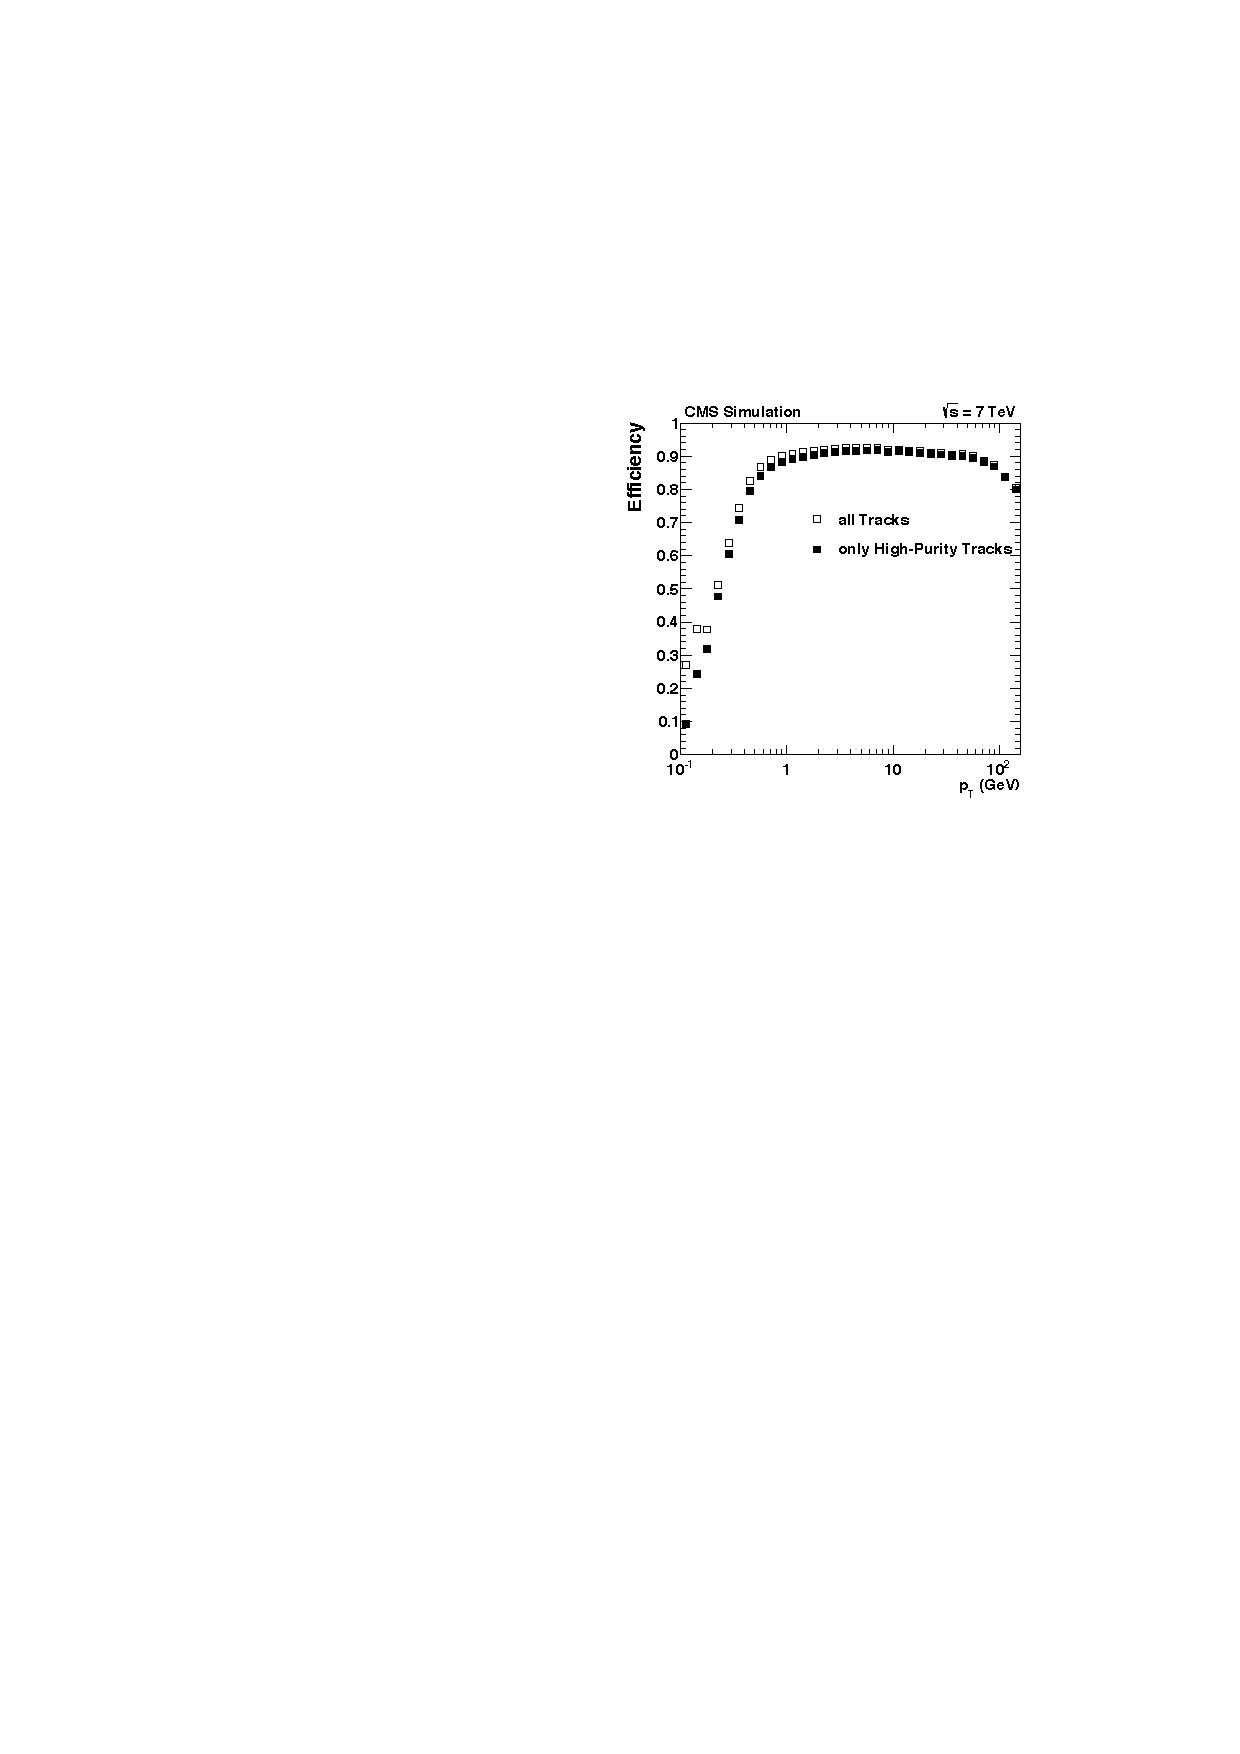
\includegraphics[width=0.5\textwidth]{3_Evt_Reconstruction/pics/trackeff.pdf}
\caption{Efficiency of the track reconstruction algorithm as a function of the particle $p_T$. It is obtained using a sample of simulated top pair events with an average number of simultaneous p-p collisions equal to 8.  
\label{fig:tracking_eff}}
\end{center}
\end{figure}


\subsection{Reconstruction of muon tracks} 

Muons can be considered a special case of the tracking algorithm, given the dedicated tracking system located outside of the solenoidal magnet. This additional lever arm allows to achieve a very good momentum resolution above 200 GeV, where the inner tracker resolution begins to degrade. 
In CMS, the muon reconstruction is seeded both by the tracker and by the muon chambers. In the former case every track above a few GeV is considered a potential muon and a tentative match with hits in the muon system is performed. If the match succeeds, the track is refitted and it acquires the status of \emph{tracker muon}. In the latter approach, a track is reconstructed by the CTF using only hits in the muon system. These tracks are seeded by track segments reconstructed by L1 trigger electronics. These \emph{standalone muons} tracks are then propagated inside the inner tracker to match with a track. As in the previous method, a successful match causes the full trajectory to be refitted and the combined object is called a \emph{global muon}. Tracker muon reconstruction is obviously more efficient than the latter for low \pT muons as they may not leave enough hits in the muon chambers to preform a full track reconstruction, but it also suffers from a larger fake rate. The two muon collections are then merged into a single one, removing double candidates.

\section{Vertex reconstruction}

Vertices are reconstructed in CMS by a \emph{Deterministic Annealing} (DA) \cite{IEEE_DetAnnealing} clustering algorithm. The tracks used during vertex reconstruction are preselected according to their transverse impact parameter with respect to the beam spot, the number of hits and the $\chi^2$\ of the track fit, to ensure that only good prompt tracks are used in the vertex reconstruction. No requirement on the track \pT is imposed in order to maximize the reconstruction efficiency in events with very little transverse momentum transfer between the colliding protons, called \emph{minimum bias} events, which compose the majority of of pile-up interactions.

Once the tracks are selected, further computations are based on the $z$\ coordinate of the points of closest approach between the tracks and the beamspot ($z_i^T$), and its uncertainty ($\sigma_i^Z$). In the DA framework the vertex position is evaluated by minimizing a modified version of the $\chi^2$\ with an additional term inflating $\sigma_i^Z$\ of each track. This parameter is called ``temperature'' since it behaves as the physics observable in statistical mechanics, with the  $\chi^2$\ acting as free energy.

Starting from one single vertex located centrally, the temperature is iteratively lowered and the free energy term minimized for each iteration. As the temperature lowers, some tracks start being incompatible with the only available vertex and a better minimum is found by splitting the tracks in two subsets belonging to two different vertices. This splitting is done ``softly'', i.e. each track can be assigned to multiple vertices with a weight between 0 and 1. With the lowering of the temperature the weights tend to assume values increasingly closer to the end-points.

The annealing process is continued down to a minimal temperature, which ensures good vertex resolution and very limited risk of splitting true vertices. After this threshold no more vertex splittings are allowed, but the temperature is still iteratively reduced and potential outliers in the vertex fits are removed. Once the final temperature ($T=1$) is reached, tracks are assigned to the corresponding vertices if their weight is greater than 0.5 as spurious weights may still be different from zero. 

Each set of tracks assigned to a vertex is then fitted with the \emph{adaptive vertex filter} algorithm \cite{CMS_NOTE_2007-008}, consisting of an iterative weighted Kalman Filter, to evaluate the vertex position with the best possible precision.

Such refined technique allows to achieve a vertex reconstruction efficiency between 98\% for cluster  of two or three tracks and 100\% for the rest, with a negligible fake rate of about 1\%. The vertex resolution for clusters of few tracks is about 200 \um both in the transverse and longitudinal plane, rapidly decreasing to an asymptotic value of about 20 \um as more tracks are used to compute the vertex position.

\section{Electron and photon reconstruction}

Both electrons and photons are reconstructed starting from ECAL clusters, which are seeded from local maxima in the energy deposition. A cluster size of $5\times5$\ crystals on average contains 95\% of the energy of an unconverted photon. This average value is considerably reduced in the real environment due to photons converting into $e\+e\-$ pairs when traversing the material in front of the calorimeter and the $e\+e\-$ pairs being separated in the $r-\phi$\ plane by the magnetic field. Photon conversions result in wider energy clusters, elongated in the $\phi$ direction. Similar arguments can be made for electrons and positrons, that emit a sequence of \emph{bremsstrahlung} photons as they approach the surface of the calorimeter. In order to recover this energy the $5\times5$\ clusters are grouped together in \emph{superclusters} (SC), elongated in the $\phi$\ direction. A more detailed description of the clustering algorithm can be found in \cite{CMS:2006tdr1}.

The bremsstrahlung process and its intrinsic non-Gaussian energy emission makes the Kalman filter approach unsuitable. It is replaced by the Gaussian Sum Filter (GSF) \cite{gsf} which handles the energy loss properly. The usage of the GSF and its larger propagation uncertainties makes a tracker-only approach unfeasible both for reasons of computation time and of low track purity. In order to reduce the amount of fake tracks, the seeding step starts from ECAL superclusters from which two track candidates are propagated inside the tracker under both charge assumptions looking for two compatible hits in the pixel detector. After the seeding, the tracking process continues as described in the previous section with the GSF substituting the KF. This modified version of the tracking algorithm is also used to correctly identify photon conversions within the tracker volume, looking for highly displaced vertices compatible with a massless state and matching a broad supercluster in the electromagnetic calorimeter.

Several variables are used to discriminate between fake and real electrons, such as the supercluster shape, its energy and location with respect to the impact position in the calorimeter, expected from the measured track parameters, and the presence of energy deposits in the hadronic calorimeter. All these variables are combined to perform the electron identification. Several working points, both with cut-based and MVA-based approach are available. The latter exploits TMVA's \cite{TMVA} Boosted Decision Tree (BDT) implementation to separate electrons from charged hadrons and photons. The BTD behavior has been trained on real electrons selected from a $\Z \To ee$ sample and fake ones from a $\Z \To ee + Jets$ one.

Photon identification is based on the same supercluster quantities as the electron identification but doesn't require a charged track to be matched to the ECAL energy deposit.  

\section{Particle Flow}


The redundancy of signals that particles traversing the CMS detector leave in multiple sub detectors is exploited by the \emph{Particle Flow} (PF) algorithm in order to improve the overall description of the event. The particle flow method furthermore allows for cross-cleaning of spurious signals and achieve to a global description of the event.

Building blocks for the PF algorithm are the different types of track collections plus the calorimeter energy deposits. Local maxima in the calorimeter deposits serve as seed for ``topological clusters'' which are grown iteratively, by adding adjacent cells with an energy deposit above a customizable threshold. After the clustering stage the algorithm links the different blocks according to their position in the $\eta-\phi$\ plane. Tracks are considered linked to calorimeter clusters if the track trajectory propagated to the average shower depth falls within the cluster boundaries, within some distance that accounts for resolution effects. Calorimeter clusters are linked if the center of the inner cluster fits within the boundaries of the outer one. The radial ordering of the linking step reflects the higher spatial resolution of the inner calorimeters (pre-shower, ECAL, HCAL). After the linking step is completed, the algorithm starts building the final objects, starting with muons. Each global muon that has a combined momentum measurement compatible with the track reconstructed in the inner detector is called a \emph{PF muon}. The corresponding track is removed from the track collection and an estimate of the associated energy deposit in the calorimeter is also removed from the list of linked clusters. Electrons are the second category of objects that is built with the procedure detailed above. Tangents to the electron trajectory in correspondence of the tracker layers are propagated to the ECAL in search for bremsstrahlung photons. If the electron candidate passes the selection cuts a \emph{PF Electron} is created and the track as well as the ECAL deposits linked to the track are removed. A tighter selection is performed on the remaining tracks, requiring that the tracker \pT resolution is smaller than the calorimetric energy resolution. This requirement is found to reject about 0.2\% of tracks in hadronic jets, 90\% of which being fake tracks. 
%Nonetheless this requirement was found to be a issue for hadronic tau reconstruction for high \pT taus and a custom modification was introduced. 
The algorithm finally exploits the redundancy in the transverse momentum measurement performed by the tracker and by the calorimeter to build \emph{PF charged hadrons, photons and neutral hadrons}. The PF algorithm operates under the assumption that all the hadrons (charged and neutral) traversing the detector are pions. Photons and neutral hadrons are produced from the calorimetric energy in the clusters once the energy of the linked tracks is subtracted. In the rare case that a calorimetric cluster has a total energy that is incompatible and lower than the sum of the linked tracks a dedicated procedure aimed at recovering mis-reconstructed muons is performed, recovering muon identification efficiency at no expense of increasing the fake rate.% Finally, to each PF object is assigned a PDG identification number and a mass.

\subsection{Muon identification}

The muon identification step in the PF reconstruction is necessary in order to suppress the hadronic punch-through, i.e. very energetic charged pions passing through the hadronic calorimeter and reaching the innermost muon station. %, and the in--flight decay of pions. 
The work presented in this thesis uses the tight working point of the PF muon identification, also referred to as ``PFTight'' within CMS.
The corresponding selection cuts are:

\begin{itemize}
\item The candidate muon must be reconstructed both as global and PF muon;
\item The normalized $\chi^2$\ of its global track fit must be less than 10;
\item There must be a least one DT or CSC hit included in the global fit;
\item At least two muon stations must be matched to the candidate;
\item The associated tracker track must have a transverse impact parameter $\mathrm{d}_{xy} < 2$\ mm and a longitudinal distance $\mathrm{d}_{xy} < 5$\ mm;
\item It must have at least one hit in the pixel detector and more than 5 hits in the whole tracker.
\end{itemize}

\subsection{Isolation}

A large fraction of the leptons produced in a proton-proton collision are due to the decay of mesons within jets. In order to separate these leptons from the ones which originate from the decay of a heavy resonance it is important to quantify the \emph{isolation} of the lepton, i.e. the amount of hadronic activity surrounding the lepton trajectory in a cone of a certain radius. The isolation can be computed separately with respect to charged and neutral particles. 

While the effect of pileup can be easily removed from the charged isolation by using only tracks associated to the selected primary vertex, the same is not possible for the neutral component. In fact calorimeters do not have sufficient spatial resolution to uniquely associate each cluster to a certain interaction vertex. The contribution of pileup to the neutral isolation is estimated by computing the energy deposited by charged tracks from pileup (i.e. not assigned to the hard-scatter vertex) and correcting it for a factor 1:2 to account for the amount of neutral energy with respect to charged one. This estimate is called \emph{$\Delta\beta = I^{pileup}_{charged}/2$}. To limit the effect of statistical fluctuations in the charged to neutral ratio on event-by-event basis the $\Delta\beta$\ correction is capped to the neutral isolation value. The \emph{relative isolation}, i.e. the isolation divided by the \pT of the object, can therefore be written as

\begin{equation}
I_{rel} = \dfrac{I_{abs}}{\pt} =  \dfrac{\sum{p_{T charged}} + \operatorname{max}(\sum{E_{T neutral}} - \D \beta, 0)}{p_T}.
\label{eq:db_rel_iso}
\end{equation}

\subsection{Jet clustering}

The particles reconstructed by the PF algorithm are clustered into jets using the \emph{Anti-kT} \cite{Cacciari:2008gp} algorithm. The Anti-kT belongs to the family of sequential recombination algorithms together with the Cambridge-Aachen and the kT algorithm \cite{Ellis:1993tq,Dokshitzer:1997in}. All these algorithms require the definition of the distance measure between two objects (in this case PF particles) and of the distance from the beam axis. In case of the Anti-kT algorithm, the distance between two objects is defined as:

\begin{equation}
d_{ij} = \operatorname{min}(\dfrac{1}{p_{Ti}^2},\dfrac{1}{p_{Tj}^2})\dfrac{\Delta R_{ij}^2}{r^2},
\end{equation}

where $r$\ is a constant parameter defining the size of the jet cone and $\Delta R = \sqrt{\Delta \eta^2 + \Delta \phi^2}$.
The distance of an object from  the beam is defined as:

\begin{equation}
d_{iB} = \dfrac{1}{p_{Ti}^2}.
\end{equation}

The algorithm starts with a high-\pT object used as seed and then it clusters around the seed all other objects until the minimum distance between the candidate jet and the closest object is larger than $d_{iB}$. One can show that this algorithm is infra-red safe, meaning that the jet shape and energy do not depend strongly on the energy of low--\pT particles clustered around a high \pT object. The Anti-kT algorithm gives rise to almost--conical jets of size $r$\ in angular aperture. Special cases are overlapping jets and jets with multiple high \pT objects within the angular acceptance.

The jets used in this work have been reconstructed with the Anti-kT algorithm with a radius parameter $r=0.5$ and their energies have been corrected to account for non-linear response of calorimeters and other instrumental effects \cite{Chatrchyan:2011ds}.

Pileup interactions deposit a considerable amount of energy in the detector. %this energy can easily overlap among different vertices and 
Furthermore, the energy deposits due to different pileup interactions may overlap and be misinterpreted by the Anti-kT algorithm as one hard jet. The CMS experiments exploits a combination of tracking and jet shape variables to discriminate between pileup jets and jets originating from the hard scattering. The information provided by these variables is interpreted by a BDT 
trained on simulated $\Z\To\mu\mu$ events \cite{CMS-PAS-JME-13-005}. The training is divided in four different $|\eta|$\ categories that reflect the resolution of tracking information and granularity of the calorimeters.

\subsection{Missing transverse energy}

%Most of the particles produced in a p-p collision leave a signal in at least one sub-detector except 
Neutrinos and other hypothetical (not yet observed) weakly--interacting particles that are neutral and stable leave no trace when traversing the detector and hence can not be directly reconstructed. Their presence can be inferred by utilizing the conservation of transverse momentum in the event. The observable quantifying an observed imbalance is called \emph{missing transverse energy} (\MET). It is computed as the negative vectorial sum of all the PF objects reconstructed in the event \cite{CMS-PAS-JME-13-003}: 

\begin{equation}
\vec{\cancel{E}_T} = -\sum^{PF\;obj.} \vec{p_{T}}
\end{equation}

The magnitude of the \MET is found to be underestimated for various reasons including thresholds in the calorimeter clustering and signal non-linearities. This bias is significantly reduced in case the correction to jet energies are included in the formula \cite{Chatrchyan:2011ds}, obtaining the ``type 1''-corrected \MET. The introduction of jet energy corrections (JEC) is performed by subtracting the vectorial residuals between all corrected and uncorrected jets found in the event:

\begin{equation}
\vec{\cancel{E}_T^{corr}} = \vec{\cancel{E}_T } - \sum_\mathrm{jets} (\vec{p}_\mathrm{T,jet}^\mathrm{corr}-\vec{p}_\mathrm{T,jet})
\label{eq:Type1MET}
\end{equation}

Additional corrections, named ``type 0'' and ``$\phi$'', correct for biases induced by pileup and by asymmetries in the $\phi$\ direction \cite{AN-13-233}.

\section{Tau reconstruction and identification}
\label{sec:tau_id}

Hadronic taus are one of the highest level objects reconstructed from CMS data and the last in the event reconstruction chain. The reconstruction and identification algorithm exploits all the detector capabilities and the Particle Flow algorithm to achieve a reconstruction efficiency close to 60\% with a sub-percent fake rate. The tau reconstruction algorithm used in CMS is called \emph{Hadron Plus Strip} (HPS) \cite{CMS-PAS-TAU-11-001,AN-14-008}. 

\subsection{Reconstruction}

Tau reconstruction is seeded from PF jets clustered by the Anti-kT algorithm with $r = 0.5$. In order to recover most of the photon conversions, the tau reconstruction algorithm clusters PF electromagnetic objects (electrons and photons) with deposited energy above 0.5 GeV in topological ``strips'' of size $0.05 \times 0.20$\ in $\eta$\ and $\phi$ direction, respectively. Strips satisfying a minimum transverse energy of 2.5 GeV are combined with the charged hadrons to form the tau candidate. The charged hadrons included in the tau reconstruction must satisfy the following requirements:

\begin{itemize}
\item $\pt > 0.5$\ GeV;
\item track fit $\chi^2 < 100$;
\item track transverse distance of closest approach to the PV $d_0 < 0.03$\ cm;
\item track longitudinal distance of closest approach to the PV $d_z < 0.4$\ cm;
\item At least three hits in the tracker.
\end{itemize}

The algorithm builds all possible combinations of hadrons plus strips matching one of the following decay modes:

\begin{enumerate}
\item \emph{single hadron}: corresponding to a single hadron and no strip.
\item \emph{hadron plus one strip}: the invariant mass of the pair has to be compatible with the $\rho$\ meson, $0.4 < M_{\tau \; candidate} < 1.3 \cdot \sqrt{\pt \mathrm{[GeV]} / 200}$\ GeV. The upper boundary of this window is limited at 1.3 (2.1) GeV for candidates with $\pt < 200 \, (> 800)$. The increasing window size accounts for resolution effects at high \pT.
\item \emph{hadron plus two strips}: the invariant mass of the triplet has to be compatible with the $\rho$\ meson, $0.4 < M_{\tau \; candidate} < 1.2 \cdot \sqrt{\pt \mathrm{[GeV]} / 200}$\ GeV. The upper boundary of this window is limited at 1.2 (2.0) GeV for candidates with $\pt < 200 \, (> 800)$.
\item \emph{three hadrons}: the invariant mass of the triplet must be compatible with the $a_1$\ meson, $0.8 < M_{\tau \; candidate} < 1.5$\ GeV. The tracks are required to be compatible with originating from the same vertex and to sum to unit charge.
\end{enumerate}

In addition the previous requirements, tau constituents are required to be contained within a cone of size 0.1, $3 / \pt \mathrm{[GeV]}$\ or 0.05 for tau candidate with $\pt < 30$ GeV, $30 < \pt < 60$ GeV and $\pt > 60$ GeV, respectively. If more than a tau candidate can be formed within the same jet only the candidate with the largest \pT is kept.

\subsection{Identification}

Hadronic tau decays reconstructed by the HPS algorithm are %identified according to their isolation within the seeding jet. 
required to be isolated in order to suppress fakes due to quark and gluon jets. Only charged hadrons with \pT above 1 GeV and photons with $E_T$\ above 1.5 GeV are considered when computing the isolation. To mitigate the effect of pileup the neutral isolation is corrected with the $\D\beta$\ method computed in a cone of $\Delta R = 0.8$ around the tau candidate. The mismatch in the size of the isolation cone ($0.5$) and the one in which the pileup contribution is computed (0.8) leads to a conversion factor from charged pileup to neutral pileup isolation of 0.4576 that is empirically found to make the tau identification efficiency insensitive to pileup.

Three working points are provided: loose, medium and tight, corresponding to isolation thresholds of 2.0, 1.0 and 0.8 GeV respectively.

%An MVA-based discrimination exploiting tau kinematic variables and isolation as well as transverse inpact parameter is also provided, but is not used in this work.

\subsection{Light lepton rejection}

The PF charged--hadron collection may contain a significant amount of electrons and muons that don't pass the selections to enter the PF electron and muon collections, and therefore are considered to be charged hadrons by the tau reconstruction algorithm. Electrons and muons from the decay of W and Z bosons are typically isolated. 
As a consequence, the background due to $e\To\tau_h$\ and $\mu\To\tau_h$\ fakes may be sizable. %The combination of this two effects causes a relatively large $e\To\tau_h$\ and $\mu\To\tau_h$\ fake rates, especially in the single hadron (muon and electrons) and in the hadron plus one strip (electrons only) decay modes. 
In order to reduce these backgrounds, dedicated discriminators against electrons and muons have been developed \cite{AN-12-417}.

\paragraph{Electron rejection:} The rejection of electrons is performed with the aid of a boosted decision tree. Tau candidates are classified into different categories depending on:

\begin{itemize}
\item The decay mode in which the tau candidate is reconstructed. Three decay modes are considered: single hadron, hadron plus one or two strips, and three hadrons. The three hadrons decay mode always passes the electron rejection discriminator;
\item Whether the hadron is associated to a track reconstructed by the GSF algorithm;
\item Whether a GSF electron candidate is reconstructed in the same direction as the tau candidate within a distance $\Delta R < 0.3$;
\item Whether the tau candidate is reconstructed in the ECAL barrel ($|\eta| < 1.479$) or endcap ($|\eta| > 1.479$).
\end{itemize}

All the possible combinations of the previous cases are considered, leading to a total of 16 mutually exclusive categories. Each category is trained separately using a mixture of  simulated events containing both signal and background processes: $\Z/\gamma^*\To\tau\tau$, $\Z/\gamma^*\To ee$, $\W\To \tau\nu$, $\W\To e\nu$, $t\anti{t}$, $H\To\tau\tau$, $\Z'\To\tau\tau$, $\Z'\To ee$, $\W'\To \tau\nu$, $\W'\To e\nu$. Events are considered as ``signal'' or ``background'' depending on whether the tau candidate is matched to a generator-level hadronic tau decay or an electron within a cone of size $\D R < 0.3$, respectively. 

%MVA training variables can be divided into four groups and are used in the training depending on the category whenever possible. The variables are summarized below.
The input variables to the BDT can be divided into four groups. The variables are:

\bold{Hadronic tau variables} (available for all categories):
\begin{itemize}
\item Invariant mass, \pT and \Eta of the tau candidate;
\item Ratio of ECAL to the sum ECAL plus HCAL energy deposits of the tau constituents;
\item Ratio of ECAL plus HCAL energy deposits of the tau constituents to the tau candidate \pT;
\item $\D\eta$\ between the tau candidate and the closest ECAL crack;
\item $\D\phi$\ between the tau candidate and the closest ECAL crack (used for candidates in the ECAL barrel only).
\end{itemize}

\bold{Strip variables} (available for taus reconstructed in the decay modes hadron plus one strip or hadron plus two strips only):
\begin{itemize}
\item $\sqrt{\pt^{\gamma} \cdot (\Delta\eta)^{2}}$\ and $\sqrt{\pt^{\gamma} \cdot (\Delta\phi)^{2}}$, 
  the \pT--weighted RMS of distances along $\eta$\ and $\phi$\ direction between all photons included in any strip and the charged hadron;
\item Fraction of $\tau_{h}$\ candidate energy carried by photons.
\end{itemize}

\bold{GSF track variables} (available only when the charged hadron is associated to a GSF track):
\begin{itemize}
\item $\ln (\pt)$, $\eta$ and normalized \chisq of the GSF track;
\item PF electron MVA output for the PF charged hadron;
\item $(N_{hits}^{GSF} - N_{hits}^{KF})/(N_{hits}^{GSF} + N_{hits}^{KF})$, where $N_{hits}^{GSF}$\ and $N_{hits}^{KF}$\ are the number of tracker hits associated to the GSF and KF tracks, respectively;
\end{itemize}

\bold{GSF electron variables} (only available in case a GSF electron is found near the hadronic tau candidate):
\begin{itemize}
\item The ratio between the total ECAL energy and the electron momentum measured at the IP;
\item Normalized \chisq, $\ln (\pt)$, $\eta$, \pT resolution ($\sigma_{\pt}/\pt$), and numbers of hits in the tracker of the electron GSF track;
\item The ratio between the bremsstrahlung photon energy as measured by the ECAL and by the track, $\sum E_{\gamma}/(P_{in}-P_{out})$, where $P_{in}$ is the momentum at the interaction vertex and $P_{out}$ is the one on the ECAL surface;
\item $F_{brem}=(P_{in}-P_{out})/P_{in}$, the ratio between the bremsstrahlung photon energy as measured by the track and the electron momentum measured at the IP;
\end{itemize}

Four working points are defined: \emph{loose }, \emph{medium}, \emph{tight} and \emph{very tight}, nominal efficiency ranging from 95\% to 80\% in steps of 5\% and corresponding decreasing $e \To \tau_h$ fake rate. %For each working point a set of different thresholds for each category is obtained by a recursive optimization. Starting from the tightest possible value (threshold set at 1 for each category), the algorithm progressively lowers the requirement in the category that allows for the highest gain in efficiency over fake-rate. The procedure is repeated until the desired fake rate is obtained.

\paragraph{Muon rejection:} uses a cut-based approach, looking for segments in the muon chambers near the direction of %muon signatures in the surroundings of 
the tau. Two working points are provided:

\begin{itemize}
\item \bold{Loose}: tau candidates are rejected if track segments in at least two muon stations are found within $\Delta R < 0.5$ or if the sum of ECAL and HCAL energy deposits associated to the leading charged hadron are less than 20\% of the momentum of its associated track.
\item \bold{Tight}: in addition to the loose working point selection no hits in the two outermost muon stations have to be found in a cone of $\D R = 0.5$\ from the tau direction.
\end{itemize}

\subsection{Performance}

\subsubsection{Identification efficiency}
\label{sec:tauid_eff}
The hadronic tau identification efficiency has been measured in 2011 data using an integrated luminosity of 1.2 fb\Inv collected at $\sqrt{s}=7$ TeV. 
The measurement was part of the PhD work presented in this thesis and was based on a \emph{tag-and-probe} method applied to $\Z\To\tau_\mu\tau_h$\ events, where $\tau_\mu$ indicates $\tau\To\mu\nu_\mu\nu_\tau$. 

Events used for the efficiency measurement have been selected as follows:
\begin{itemize}
\item The event is required to have fired the single-muon trigger path with $\pt^\mu > 17$ GeV. The chosen trigger path prevents any bias on the hadronic tau leg selection, while the \pT threshold corresponds to the lowest unprescaled single muon trigger path for the analyzed run period;
\item The event must contain at least one vertex with $\geq 4$\ degrees of freedom, reconstructed within 24 cm along $z$\ from the nominal interaction point and within 2 cm in the transverse plane from the beamspot position;
\item The event must contain one muon with $\pt > 20$\ GeV and $|\eta| < 2.1$, with a relative isolation below 0.3 in a cone of $\D R < 0.4$ (no \db corrections to the muon isolation are applied);
\item The event must contain a tau-jet candidate with $\pt > 20$\ GeV and $|\eta| < 2.3$. In order to reject electrons and muons being identified as tau-jet candidates it has to be separated from any segment in the muon system by $\D R > 0.5$\ and to be identified as hadron-like by the PF electron and photon MVA identification. In addition, the \emph{leading} (highest \pT) object in the tau-jet candidate is required to be a charged hadron with $\pt > 5$\ GeV and the \pT sum of charged and photon PF objects in an annulus of size $0.15 < \D R < 0.6$\ around the leading track must be below 2.5 GeV. These last two requirements are found to significantly reduce the backgrounds while having a high efficiency for genuine taus;%little influence on the outcome of the measurement; 
\item A veto on any additional global muon is imposed on the event.
\end{itemize}

Events passing the previous selection are then divided into six mutually-exclusive categories (called A, B, C1p, C1f, C2, and D). C1p and C1f categories contain $\Z\To\tau_\mu\tau_h$\ events where the \tauh\ passes or fails the hadronic tau identification criteria, respectively. The other categories are dominated by the two main backgrounds to this analysis, $\W+Jets$ and QCD events, and are used in a simultaneous fit to constrain the yields of these to backgrounds in the signal region.
Events are assigned to the proper category as follows: % according to the following event properties:
\begin{itemize}
\item In the C1p, C1f, C2, and D categories the muon relative isolation is required to be below 0.1;
\item In the C1p, C1f, C2, and A categories the muon and the tau-jet leading track are required to be of opposite charge;
\item In the C1 categories it is required that $M_T(\mu, \vecmet) < 40$\ GeV and that $\pz -1.5 \cdot \pz^{vis} > -20$\ GeV, where:

\begin{equation}
 M_T(\mu, \vecmet) = \sqrt{(E_{T}^\mu+\met)^2 - (\vec{\pt^\mu}+\vecmet)^2}
\end{equation}
\begin{equation}
 \pz = (\vec{\pt^\mu} + \vec{\pt^{\tau\,jet}} + \vec{\cancel{E}_T}) \cdot \vec{\zeta}
\end{equation}
\begin{equation}
 \pz^{vis} = (\vec{\pt^\mu} + \vec{\pt^{\tau\,jet}}) \cdot \vec{\zeta}
\end{equation}

where $\vec{\zeta}$\ is the versor bisecting the angle between the muon and the tau-jet candidate in the transverse plane \cite{CDFrefPzeta}.%two visible transverse momenta;
\item The categories C1p and C1f contain the events where the tau-jet candidate passes or fails the tau identification working point, respectively.
\end{itemize}

A graphical illustration of the event categories is shown in Figure \ref{fig:tau_eff_ABCD}.

\begin{figure}
\begin{center}
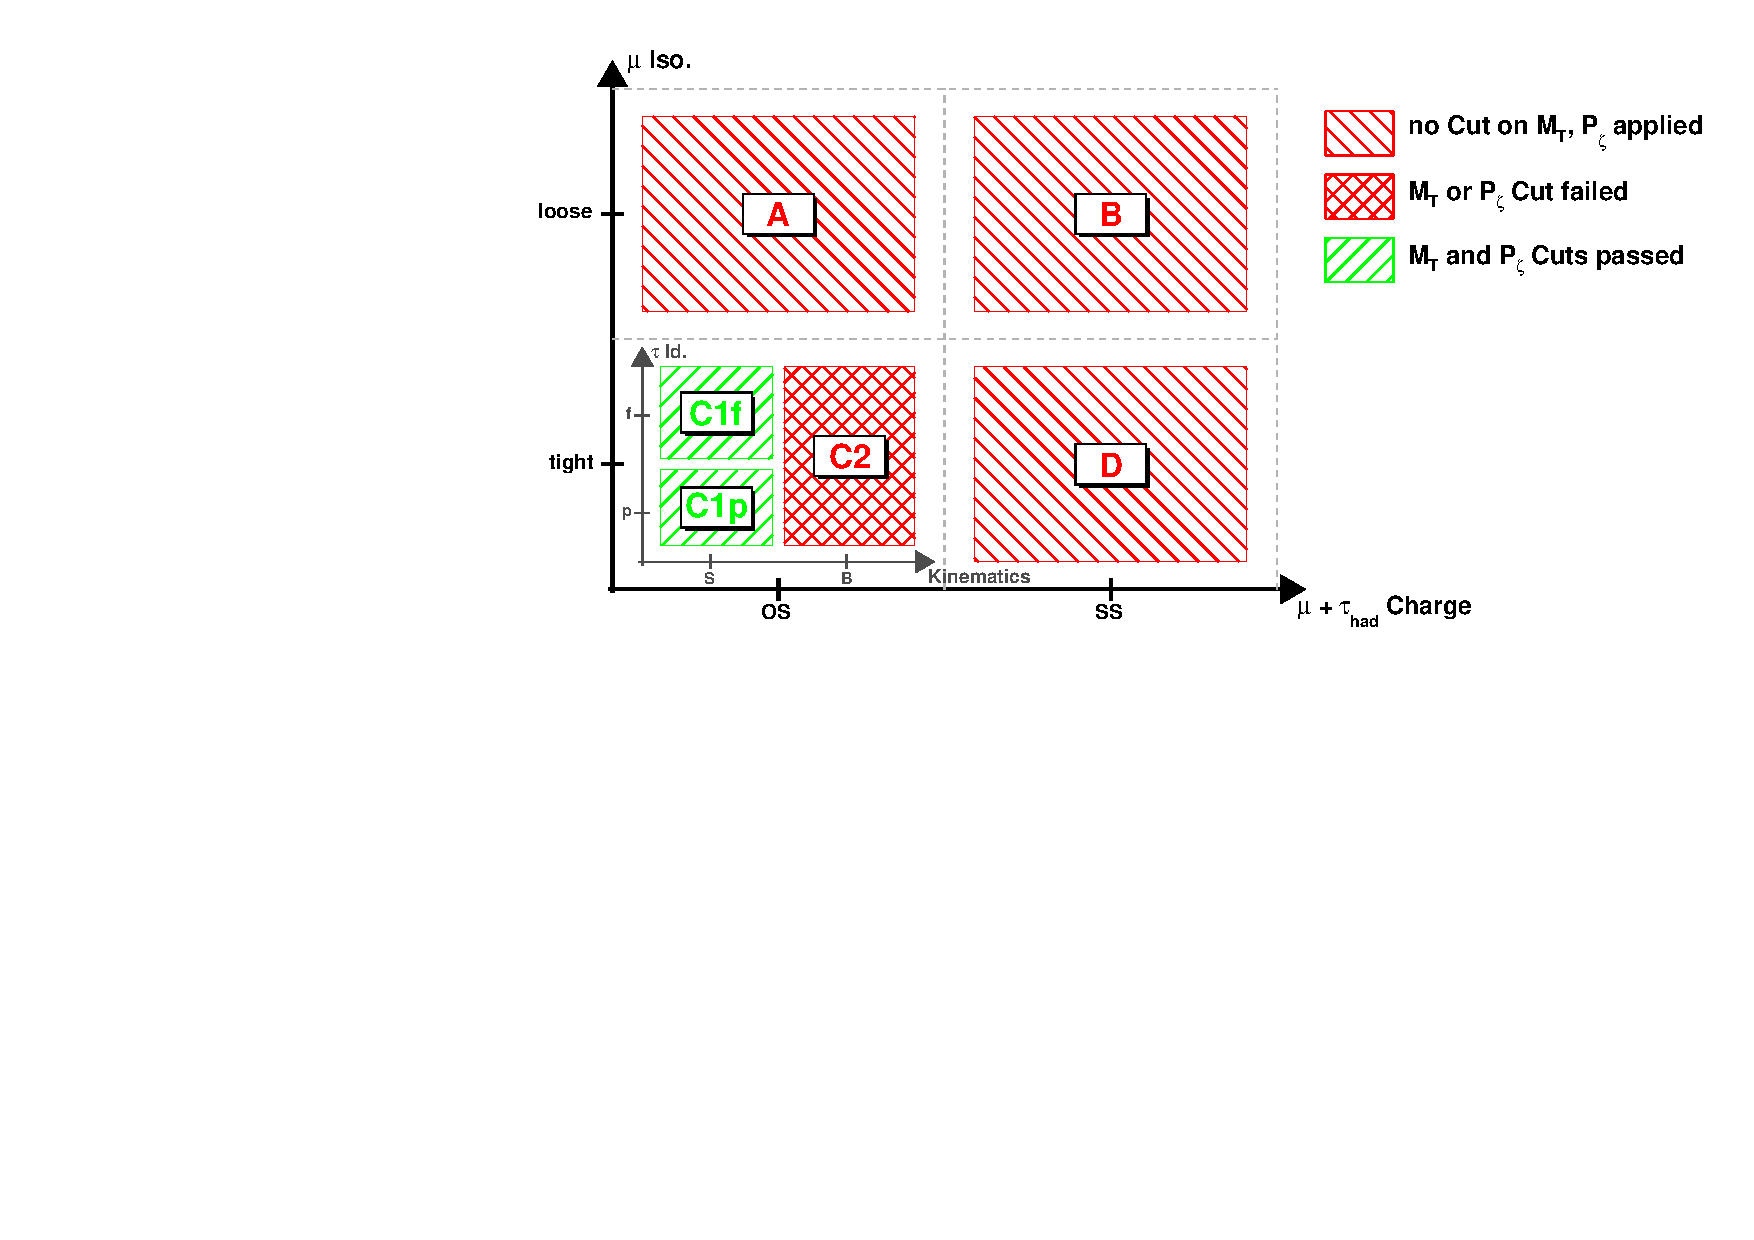
\includegraphics[angle=-0,width=0.8\textwidth]{3_Evt_Reconstruction/pics/figTauIdEffIllustration.pdf}
\caption{Illustration of signal and control regions used in the efficiency measurement and their requirements.
\label{fig:tau_eff_ABCD}
}
\end{center}
\end{figure}

The processes considered signal and background in the tau identification efficiency measurement %as contributing in the defined regions 
are: $\Z\To\tau\tau$, $\Z\To\mu\mu$, $\W\To\ell\nu+\rm{Jets}$, $t\anti{t}+\rm{Jets}$\ and QCD multijet production processes. All the kinematic distribution shapes used for this processes in the analysis are taken from MC simulation and normalized to the NLO predictions with the exception of the QCD shape in the C1p and C1f regions, where, to mitigate the lack of MC statistics, the shape is taken from the data distribution in the B region with the additional requirements of $M_T < 40$\ GeV and $\pz -1.5 \cdot \pz^{vis} > -20$. 

The yield of each process contributing to the measurement is expressed as a product of the total yield ($N^i$), the probability to pass (or fail) the muon isolation ($p_{\mu\,\rm{Iso}}^i$), the probability to pass (or fail) the leading track charge requirement ($p_{ch}^i$), the probability to pass (or fail) the topological cuts ($p_{topo}^i$) and the probability pass (or fail) the given tau-identification discriminator, $p_{\tau ID}^i$. The parameters listed above, initialized to their MC expectation, are inferred from data with a simultaneous template fit of all the regions and the different signal and background components. The physical observables used for the template fit is the invariant mass of the visible decay products, also called \emph{visible mass}, ($M_{vis}$), for the C1p and C1f categories and the transverse mass of the muon and \MET for the others. Figure \ref{fig:TauID_2011_fits} shows the results of the template fit for the loose discriminator.

\begin{figure}
	\setlength{\unitlength}{1mm}
	\begin{center}
		\begin{picture}(150,170)(0,0)
			\put(0.5, 118){\mbox{\includegraphics*[height=52mm]{3_Evt_Reconstruction/pics/controlPlotsTauIdEff_wConstraints_A_diTauMt_tauDiscrHPScombLooseDBcorr_all_fitted_diTauVisMass_ewkBgSum.pdf}}}
			\put(78.0, 118){\mbox{\includegraphics*[height=52mm]{3_Evt_Reconstruction/pics/controlPlotsTauIdEff_wConstraints_B_diTauMt_tauDiscrHPScombLooseDBcorr_all_fitted_diTauVisMass_ewkBgSum.pdf}}}
			\put(0.5, 60){\mbox{\includegraphics*[height=52mm]{3_Evt_Reconstruction/pics/controlPlotsTauIdEff_wConstraints_C1p_diTauVisMass_tauDiscrHPScombLooseDBcorr_passed_fitted_diTauVisMass_ewkBgSum.pdf}}}
			\put(78.0, 60){\mbox{\includegraphics*[height=52mm]{3_Evt_Reconstruction/pics/controlPlotsTauIdEff_wConstraints_C1f_diTauVisMass_tauDiscrHPScombLooseDBcorr_failed_fitted_diTauVisMass_ewkBgSum.pdf}}}
			\put(0.5, 2){\mbox{\includegraphics*[height=52mm]{3_Evt_Reconstruction/pics/controlPlotsTauIdEff_wConstraints_C2_diTauMt_tauDiscrHPScombLooseDBcorr_all_fitted_diTauVisMass_ewkBgSum.pdf}}}
			\put(78.0, 2){\mbox{\includegraphics*[height=52mm]{3_Evt_Reconstruction/pics/controlPlotsTauIdEff_wConstraints_D_diTauMt_tauDiscrHPScombLooseDBcorr_all_fitted_diTauVisMass_ewkBgSum.pdf}}}
			\put(-5.5, 170.5){\small (A)}
			\put(72.0, 170.5){\small (B)}
			\put(-5.5, 112.5){\small (C1p)}
			\put(72.0, 112.5){\small (C1f)}
			\put(-5.5, 54.5){\small (C2)}
			\put(72.0, 54.5){\small (D)}
		\end{picture}
		\caption{
         Measured distributions of $M_{T}$\ for the regions $A$, $B$, $C2$\ and $D$\ and of $M_{vis}$\ for $C1p$\ and $C1f$\ compared to the sum of templates associated to the signal and background processes. ``EWK Bgr.'' denotes the sum of $Z \to \mu^{+} \mu^{-}$\ and $W$\ + jet background contributions. The templates are scaled by normalization factors obtained by the fit for the loose working-point of the HPS combined isolation discriminator.
}
		\label{fig:TauID_2011_fits}
	\end{center}
\end{figure}


The inferred probability to pass the tau identification discriminator is related to its efficiency by:

\begin{equation}
 \epsilon_{\tau ID} = p_{\tau ID} \cdot \epsilon_f \cdot \epsilon_p \cdot \epsilon_i \cdot k_{jet \To \tau} \cdot k_p \cdot k_i
\end{equation}

Where the symbols $\epsilon$\ denote the preselection efficiencies and $k$\ the correction factors. The correction factors account for the fraction of taus that would pass the tau identification, but fail either the jet isolation ($k_i$), or the leading track requirement ($k_p$), and for the small amount of quark and gluon jets present in the $\Z\To\tau\tau$\ templates ($k_{jet \To \tau}$). These correction factors are extracted from MC simulation. 

The measured hadronic tau identification efficiency is compared to the MC prediction. %computed as a deviation from the predicted efficiency of the MC simulation. 
The efficiencies measured for all the tau identification discriminators are found to be in agreement with the MC prediction within the uncertainties, even though a small trend towards lower values may be seen for the tighter working points. The uncertainty in the efficiency for hadronic tau decays to pass the working point used in the search for the $\rm{H}\To\tau\tau$ presented in this thesis amounts to 
 6\% with an identification efficiency of roughly 60\%. The uncertainty represents the sum of statistical and systematic uncertainties added in quadrature. The main source of statistical error comes from the large uncertainties in the $\Z\To\tau\tau$ yield in the C1f region, while the leading systematic uncertainty is the reconstruction efficiency for hadronic tracks. A summary of the systematic uncertainties considered in the measurement can be found in Table~\ref{tab:tau_eff_sys}.

\begin{table}
\begin{center}
\caption{Summary of systematic uncertainties considered in the hadronic tau identification efficiency measurement, and their effect on the final result.}
\label{tab:tau_eff_sys}
\begin{tabular}{|c|c|}
 \hline
 systematic uncertainty & effect \\
 \hline
Muon momentum scale & $\ll 1\%$ \\
$\tau$--Jet energy scale & $ < 1\%$ \\
Hadronic track reconstruction & $3.9\%$ \\
Track momentum scale & $< 1\%$ \\
Loose Isolation & $2.5\%$ \\
$\rm{Jet}\To\tau_h$ fake rate & $1.2\%$ \\
$k_p$ uncertainty & $1.7\%$ \\
$k_i$ uncertainty & $2.1\%$ \\
Statistical uncertainty & $2.6\%$ \\
\hline
Total & $6.0\%$ \\
\hline
\end{tabular}
\end{center}
\end{table}


\subsubsection{Jet fake probability}

The $\rm{jet} \To \tau_h$ fake probability is measured using $\W+\rm{Jets}$ and QCD events. Events are selected online by a single--muon (W events) or single--jet (QCD events) trigger. W+Jets events are required to contain a well identified and isolated muon with $M_T(\mu, \met) > 50$ GeV. The $\rm{jet} \To \tau_h$ fake probability is computed for all taus with $\pt > 20$ GeV, $|\eta| < 2.3$ and passing the combination of ``decay mode finding'' plus the isolation discriminator under study with respect to all jets of $\pt > 20$ GeV and $|\eta| < 2.3$ \cite{DP-14-015}:

\begin{equation}
 p(jet \To \tau_h) = \dfrac{\operatorname{N}(\pt^{\tau_h} > 20\GeV \AND |\eta^{\tau_h}| < 2.3 \AND \mathrm{Decay-Mode} \AND \mathrm{Discriminator\,WP})}{\operatorname{N}(\pt^{jet} > 20\GeV \AND |\eta^{jet}| < 2.3)}
\end{equation}

The $jet \To \tau_h$ fake probability measured in W+jets events as a function of jet \pT, $\eta$, $\phi$ and as a function of the number of reconstructed vertices is shown in Figure \ref{fig:jetToTauFakeRate_Wjets_HPScombIso3Hit}. The $jet \To \tau_h$ fake probability is found to be strongly dependent to the jet \pT. An increase of the fake probability is also observed at high $\eta$ values, where the tracking efficiency decreases, affecting the discriminating power of the isolation-based discriminators. A mild dependence on the number of pileup vertices is also observed. This effect is due to the \db correction, which gradually switches off the neutral isolation discrimination as the pileup increases, leaving only the track-based isolation. Please note that the \db correction has been tuned to keep the efficiency constant as a function of the number of pileup interactions, causing the fake-rate to increase; another possible solution could have been keeping the fake-rate stable at the cost of reducing the efficiency. The slight mismatch between data and MC prediction is due to a mismodeling in the simulation of \emph{out-of-time pileup}, i.e. the effect that collisions from previous bunch crossings have in the current event. This effect is visible only in high-latency detectors such as the ECAL.

\begin{figure}
\setlength{\unitlength}{1mm}
\begin{center}
\begin{picture}(150,150)(0,0)
\put(-2.5, 74.5){\mbox{\includegraphics*[height=74mm]{3_Evt_Reconstruction/pics/jetToTauFakeRateVsPt_Wjets_HPScombIso3Hit.pdf}}}
\put(80.0, 74.5){\mbox{\includegraphics*[height=74mm]{3_Evt_Reconstruction/pics/jetToTauFakeRateVsEta_Wjets_HPScombIso3Hit.pdf}}}
\put(-2.5, -1.5){\mbox{\includegraphics*[height=74mm]{3_Evt_Reconstruction/pics/jetToTauFakeRateVsPhi_Wjets_HPScombIso3Hit.pdf}}}
\put(80.0, -1.5){\mbox{\includegraphics*[height=74mm]{3_Evt_Reconstruction/pics/jetToTauFakeRateVsNvtx_Wjets_HPScombIso3Hit.pdf}}}
\put(-5.5, 148.5){\small (a)}
\put(77.0, 148.5){\small (b)}
\put(-5.5, 72.5){\small (c)}
\put(77.0, 72.5){\small (d)}
\end{picture}
\end{center}
\caption{
  Probabilities for quark and gluon jets in $W$+jets events to pass the \emph{HPS combined isolation 3--hit}) discriminator, as function of jet $P_{T}$ (a), $\eta$ (b), $\phi$ (c) and as function of $N_{vtx}$, the number of vertices reconstructed in an event (d). The fake--rates measured in data are compared to the Monte Carlo expectation.}
\label{fig:jetToTauFakeRate_Wjets_HPScombIso3Hit}
\end{figure}


\subsubsection{Electron and Muon fake probability}

The rejection power of the anti-electron and anti-muon discriminators is computed in $\Z\To\ell\ell$ events with a tag-and-probe technique. Well identified and isolated leptons are used to select the events both online and offline. The event is required also to contain a tau candidate passing only the decay-mode finding plus loose isolation discriminators (probe). The dimuon invariant mass distribution is fitted both in regions passing and failing the anti-lepton requirement to extract the rejection power and the ratio between data and MC. 

%The achieved rejection power for the two leptons is summarized in Table \ref{tab:tau_lep_rej}

%\begin{table}
%\begin{center}
%\caption{TODO, put values!}
%\begin{tabular}{|c|c|c|}
% \toprule
% Working point & efficiency & rejection power \\
% \midrule
% \multicolumn{3}{|c|}{muon rejection} \\
% \hline
% Loose & XX\% & XX\% \\
% Tight   & XX\% & XX\% \\
% \hline
% \multicolumn{3}{|c|}{electron rejection} \\
% \hline
% Loose    & XX\% & XX\% \\
% Medium & XX\% & XX\% \\
% Tight     & XX\% & XX\% \\
% Very Tight & XX\% & XX\% \\
% \bottomrule
%\end{tabular}
%\end{center}
%\label{tab:tau_lep_rej}
%\end{table}
